
\lecture[14]{More on hypothesis testing}{lecture-text}

\subtitle{and checking conditions}

\date{20 October 2015}


\begin{document}

\begin{frame}
  \maketitle
\end{frame}


\begin{frame}{Last time}

  \begin{itemize}
    \item An \alert{observational study} observes an existing situation,
    \item to look for correlations.
    \item But, \alert{correlation is not causation},
    \item thanks in part to \alert{confounding factors}.
    \item \alert{Experimental studies} try to eliminate these,
    \item so provide much stronger evidence of causation.
  \end{itemize}


\end{frame}

\begin{frame}\frametitle<presentation>{Outline}
  \tableofcontents
\end{frame}

%%%%%% %%%%%%
\section{Significant or important?}

\subsection{Unpacking the terminology}


%%%%%%
\begin{frame}{Interpreting results}

  % \begin{quote}
  %   \textbf{Results:}
  %   According to pairwise analysis, the active twins had lower body fat percentage ($P=0.029$) and homeostatic model assessment index ($P=0.031$) and higher Matsuda index ($P=0.021$) compared with their inactive co-twins.  Striatal andprefrontal cortex (subgyral and inferior frongal gyrus) brain gray matter volumes were larger in the nondominant hemisphere in active twins compared with those in inactive co-twins, with a statistical threshold of $P<0.001$.
  % \end{quote}
  \begin{center}
    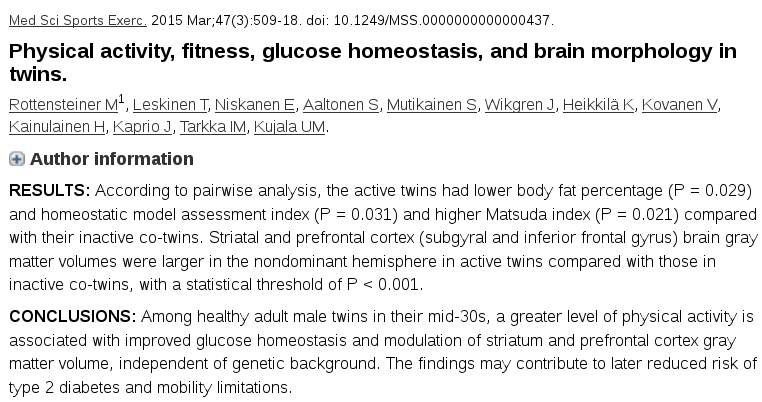
\includegraphics[width=\textwidth]{examples/twins-exercise_abstract_results}
  \end{center}
  \flushright{\small \url{http://www.ncbi.nlm.nih.gov/pubmed/25003773}}

  \vspace{2em}

  Let's unpack those statements.

\end{frame}

%%%%%%
\begin{frame}{Statistical significance}

    \begin{quote}
        had \only<2->{\alert{statistically significantly} }lower body fat percentage ($P=0.029$),
        \only<3->{\alert{at the $\alpha=0.05$ significance level}}
    \end{quote}

    \uncover<4->{
    \structure{means, roughly}
    \begin{quote}
        we found good evidence that the difference in body fat was not caused by chance variation alone
    \end{quote}
    }

    \uncover<5->{
    \structure{or more precisely}
    \begin{quote}
        if the null hypothesis was true, we'd expect to see at least this large a difference no more than 5\% of the time
    \end{quote}
    }

\end{frame}

%%%%%%
\begin{frame}{Lack of statistical signficance}

    \begin{quote}
      no \only<2->{\alert{statistically significant }}difference was found in body mass index ($P=0.28$) \only<2->{\alert{at the $\alpha=0.05$ signficance level}}
    \end{quote}

    \uncover<3->{
    \structure{means, roughly}
    \begin{quote}
        there was not sufficient evidence that the observed difference in body mass index was due to anything other than chance variation
    \end{quote}
    }

    \uncover<3->{
    \structure{or more precisely}
    \begin{quote}
        if the null hypothesis was true, we'd expect to see at least this large a difference \alert{at least} 5\% of the time
    \end{quote}
    }

\end{frame}

%%%%%%%
\begin{frame}{What do you conclude?}

    If you do a study, \\
    and someone asks you \alert{what your conclusion is},\\
    they probably want to know

    \vspace{2em}

    \begin{enumerate}
        \item What was the result?
        \item How strong was the statistical support?
        \item What are the real-world implications?
    \end{enumerate}

\end{frame}

%%%%%%%
\begin{frame}{Example}

    Sock height (in inches) from randomly chosen USC students:
  \begin{center}
    \begin{tabular}{crr}
       & Males & Females \\
       \hline
       $n$ & 27 & 26 \\
       $\bar y$ & 2.2 & 1.4 \\
       $s$ & 1.1 & 1.0
     \end{tabular}

     \vspace{1em}

     $t_s=2.3$ and $P=0.03$

     \begin{itemize}
         \item[2-] \textit{What was the result?} \\
            Males tended to have taller socks than females,
        \item[3-] \textit{How strong was the statistical support?} \\
            the difference was statistically significant ($P=0.03$),
        \item[4-] \textit{What are the real-world implications?} \\
            but the results may not apply to other groups.
     \end{itemize}

\end{frame}

%%%%%%%
\begin{frame}{Example 2}

    Infection intensity in a randomized controlled trial:
  \begin{center}
    \begin{tabular}{crr}
       & control & treatment \\
       \hline
       $n$ & 27 & 26 \\
       $\bar y$ & 2.2 & 1.4 \\
       $s$ & 1.1 & 1.0
     \end{tabular}

     \vspace{1em}

     $t_s=2.3$ and $P=0.03$

     \begin{itemize}
         \item[2-] \textit{What was the result?} \\
            The treatment group had lower mean infection intensity,
        \item[3-] \textit{How strong was the statistical support?} \\
            and there was good evidence the difference was not due to chance ($P=0.03$);
        \item[4-] \textit{What are the real-world implications?} \\
            this provides good evidence that the treatment decreases infection intensity.
     \end{itemize}

\end{frame}

%%%%%%
\begin{frame}{Practice}

  Lactate dehydrogenase levels:
  \begin{center}
    \begin{tabular}{crr}
       & Males & Females \\
       \hline
       $n$ & 270 & 264 \\
       $\bar y$ & 60 & 57 \\
       $s$ & 11 & 10
     \end{tabular}

   \vspace{2em}

   \uncover<2->{$t_s=3.3$ and $P=0.001$}
   \end{center}

   \vfill

  Body weight:
  \begin{center}
    \begin{tabular}{crr}
       & Males & Females \\
       \hline
       $n$ & 2 & 2 \\
       $\bar y$ & 175 & 143 \\
       $s$ & 35 & 34
     \end{tabular}

   \vspace{2em}

   \uncover<2->{$t_s=0.93$ and $P=0.45$}
   \end{center}

\end{frame}


%%%%%%
\begin{frame}{What do you think they did?}

    \begin{quote}
        The subjects were given varying doses of the drug and also a placebo in a double-blind randomized trial. Researchers found low doses [...] improved memory performance[.]
    \end{quote}
    \figcaption{\textit{Drug restores brain function and memory in early Alzheimer's disease}, \url{http://www.sciencedaily.com/releases/2015/03/150311124200.htm}}

    \vfill
    \pause

    \begin{quote}
        We observed significant improvement in memory task performance under drug treatment relative to placebo in the aMCI cohorts at the 62.5 and 125 mg BID doses of levetiracetam.
    \end{quote}
    \figcaption{\url{http://www.sciencedirect.com/science/article/pii/S2213158215000273}}

\end{frame}



%%%%%% %%%%%% %%%%%% %%%%%%
\section{Describing real-world importance}

%%%%%%%
\begin{frame}{Significant or important?}
    \vfill

    So you have a \alert{tiny $P$-value}.

    \vfill

    How big is the effect?

    \vfill
    \pause

    \structure{Or,} I believe your result is not noise,
    but how much \alert{do I care?}

\end{frame}

%%%%%%
\begin{frame}{It's significant, but is it important?}


    \begin{block}{the difference in means}
        We've observed a difference between two populations:
        \[  \bar y_1 - \bar y_2 \]
    \end{block}

    \ldots and got a small $P$-value.  So what?

    \vspace{2em}

    \structure{Ask yourself:} What do we want to know?\\

    \vspace{2em}

    How important is the observed difference?


\end{frame}


%%%%%% %%%%%%
\subsection{The effect size}

%%%%%%
\begin{frame}{}

    \begin{block}<1->{the $t$-statistic}
        \begin{align*}
            t_s = \frac{\bar y_1 - \bar y_2}{ \SE_{\bar Y_1 - \bar Y_2} } 
            = \frac{ \text{(actual difference)} }{ \text{(magnitude of sampling noise)} }
        \end{align*}
        is big if the observed difference is large compared to the estimated size of the \alert{estimation error}.
    \end{block}

    \begin{block}<2->{the effect size}
        If both populations have the same SD, $\sigma$,
        \begin{align*}
            \text{(Effect size)} = \frac{\bar y_1 - \bar y_2}{ \sigma }
            = \frac{ \text{(actual difference)} }{ \text{(magnitude of within-population variation)} }
        \end{align*}
        is big if the observed difference is large compared to \alert{within-population variation}.
    \end{block}

\end{frame}

%%%%%%
\begin{frame}{Examples}
    In each, 
    what are the $t$-statistics
    and the effect sizes?
    What do they tell us?

  \vfill

  Lactate dehydrogenase levels:
  \begin{center}
    \begin{tabular}{crr}
       & Males & Females \\
       \hline
       $n$ & 270 & 264 \\
       $\bar y$ & 60 & 57 \\
       $s$ & 11 & 10
     \end{tabular}
  \end{center}
  
  \vfill

  Body weight (lb):
  \begin{center}
    \begin{tabular}{crr}
       & Males & Females \\
       \hline
       $n$ & 2 & 2 \\
       $\bar y$ & 175 & 143 \\
       $s$ & 35 & 34
     \end{tabular}
 \end{center}

\end{frame}


%%%%%% %%%%%%
\subsection{Using confidence intervals}

%%%%%%
\begin{frame}{Significantly unimportant?}

    The \alert{confidence interval} describes where we are pretty confident the true value lies.

    \begin{itemize}

    \item So if we think an effect smaller than $x$ is \alert{unimportant}
      and $x$ is outside the confidence interval,

    \item then we have good evidence the true effect is unimportant.
      (inconsequential, insignificant, \ldots?)

    \end{itemize}

    \vspace{2em}

    Examples:
    \begin{itemize}
      \item Lactate dehydrogenase levels:
      \item Body weight:
    \end{itemize}

\end{frame}

%%%%%%
\begin{frame}{Interpret:}

  \begin{quote}
    ``Our data also suggest a positive association of cigarette smoking and new HPV detection (OR, 3.4; 95\% CI, 0.4--26.3); {however, because 87\% of study participants were smokers, we had limited power to detect significant effects.}''
  \end{quote}

  \vspace{2em}

  OR = ``odds ratio'' = increased odds of contracting HPV

\end{frame}


%%%%%%
\begin{frame}{Not significant, but important?}

    Recall that ``not signficant'' means
    \begin{quote}
        there was not sufficient evidence that the observed difference was due to anything other than chance variation.
    \end{quote}


    \vspace{2em}

    This does \alert{not} mean that there is no real difference!

    \vspace{2em}

    If the confidence interval includes zero, but also some big (important) values,
    then we don't have the \alert{power} to tell.  
    Here ``not significant'' reflects our uncertainty.



\end{frame}


%%%%%%
\begin{frame}{Tomato yield}

    Comparing the yield of two tomato varieties,
    a mean difference of 1 pound per plant is ``important''.

    \vspace{2em}

    \begin{center}
    \begin{tabular}{c|cc}
        95\% CI & significant? & important? \\
        \hline
        0.2 -- 0.3 & & \\
        1.2 -- 1.3 & & \\
        0.2 -- 1.3 & & \\
        -0.2 -- 0.3 & & \\
        -1.2 -- 0.3 & & \\
        \hline
    \end{tabular}
    \end{center}


\end{frame}


%%%%%%
\mode<presentation>{
\begin{frame}{Tomato yield}

    Comparing the yield of two tomato varieties,
    a mean difference of 1 pound per plant is ``important''.

    \vspace{2em}

    \begin{center}
    \begin{tabular}{c|cc}
        95\% CI & significant? & important? \\
        \hline
        0.2 -- 0.3 & yes & no \\
        1.2 -- 1.3 & yes & yes \\
        0.2 -- 1.3 & yes & don't know \\
        -0.2 -- 0.3 & no & no \\
        -1.2 -- 0.3 & no & don't know \\
        \hline
    \end{tabular}
    \end{center}


\end{frame}
}


%
\begin{frame}{What's missing?}
  \begin{center}
    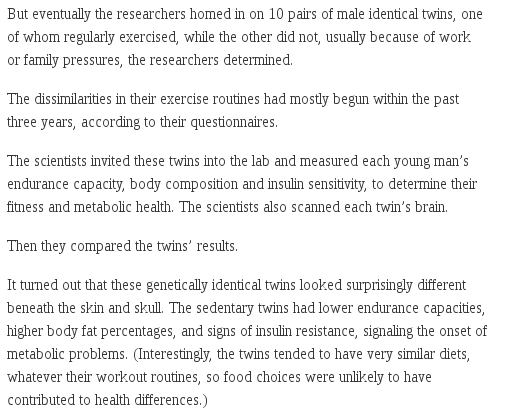
\includegraphics[width=0.85\textwidth]{examples/twins-exercise_news}
  \end{center}
  \flushright\small\figcaption{\url{http://well.blogs.nytimes.com/2015/03/04/one-twin-exercises-the-other-doesnt}}
\end{frame}

%
\begin{frame}{Is it here?}
  {\small
  ``{Physical activity, fitness, glucose homeostasis, and brain morphology in twins.}'', 
  }
  \begin{center}
    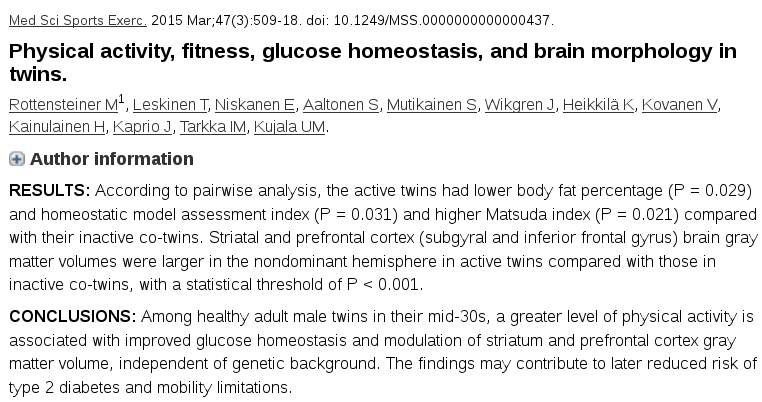
\includegraphics[width=\textwidth]{examples/twins-exercise_abstract_results}
  \end{center}
  \flushright\small\figcaption{
  ``Physical activity, fitness, glucose homeostasis, and brain morphology in twins.'', 
  \url{http://www.ncbi.nlm.nih.gov/pubmed/25003773}
  }
\end{frame}

%
\begin{frame}[plain]{The results}
  \begin{center}
    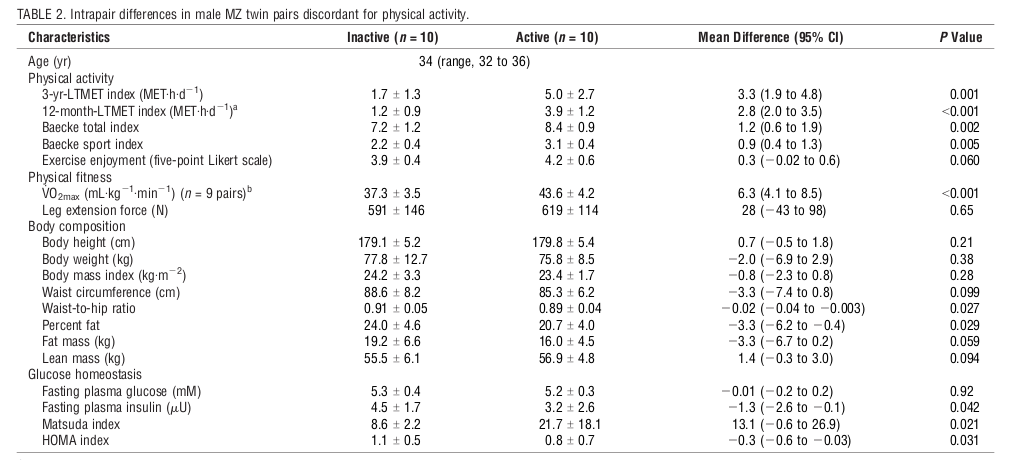
\includegraphics[width=1.2\textwidth]{examples/twins-exercise_study-results}
  \end{center}
  \flushright\small\figcaption{
  \url{http://www.ncbi.nlm.nih.gov/pubmed/25003773}
  }
\end{frame}



\section{Conditions for (best) use of a $t$-test}

\begin{frame}{What are ``conditions''?}

  Statistical tests usually work by finding the probability that 
  \begin{itemize}
    \item something happens,
    \item under a certain generative model.
  \end{itemize}

  \vspace{2em}

  \structure{Example:} The $P$-value for the $t$-test is the probability that 
  \begin{itemize}
    \item the difference in sample means between independent samples from two populations is at least as big as the observed value ($\bar y_1 - \bar y_2$), 
    \item if the two populations have the same mean ($\mu_1 = \mu_2$), and the sampling distribution of the sample mean is Normal.
  \end{itemize}

  \vspace{2em}
  
  \alert{Conditions}, a.k.a.\ ``assumptions'', come from the generative model.
  If they are not true, we might
  \begin{itemize}
    \item have \alert{wrong} $P$-values (misreport the type I error rate)
    \item \structure{and/or} have lower power than a better test \\
      (i.e.\ have more type II errors)
  \end{itemize}

\end{frame}

\subsection{The $t$-test}

%%%%%%
\begin{frame}{the $t$-test}

  \begin{block}{Conditions for the $t$-test}
    \begin{enumerate}
      \item The sampling procedure provides:
        \begin{enumerate}
          \item random, independent samples from large populations,
          \item with the two samples independent of each other.
        \end{enumerate}
      \item The sampling distributions of $\bar Y_1$ and $\bar Y_2$ are
        \begin{enumerate}
          \item close enough to Normal.
      \end{enumerate}
    \end{enumerate}
  \end{block}

  \vspace{2em}

  \structure{Red flags for the $t$-test:}
  \begin{enumerate}
    \item Nonindependence of samples
    \item Small sample sizes 
    \item Skewed distributions
  \end{enumerate}

  \vspace{2em}

  ``Small'' means less than around 20,
  but depends on how close the population distribution is to Normal.

\end{frame}

%%%%%%
\begin{frame}{Simple example}


  \vspace{2em}


  Body weight:
  \begin{center}
    \begin{tabular}{crr}
       & Males & Females \\
       \hline
       $n$ & 2 & 2 \\
       $\bar y$ & 175 & 143 \\
       $s$ & 35 & 34
     \end{tabular}

   \vspace{2em}

   {$t_s=0.93$ and $P=0.45$}\\
   CI for $\bar \mu_1 - \bar \mu_2$: $(-117,181)$
   \end{center}

   \vspace{2em}
  
   \pause
   \alert{The sample sizes are too small} to take the statistics seriously.
   
\end{frame}


%
\begin{frame}{Example: earthquakes}

  % > do.call( cbind, with( subset(quakes,MAG>3), tapply( MAG, weekdays(date), function (x) { list(n=length(x),mean=mean(x),sd=sd(x)) } ) ) )
  %      Friday    Monday    Saturday  Sunday    Thursday  Tuesday   Wednesday
  % n    21        24        31        22        23        24        21       
  % mean 3.33381   3.433333  3.509677  3.309545  3.49913   3.29125   3.382857 
  % sd   0.2215508 0.3715732 0.5015409 0.3381388 0.4162376 0.2501706 0.3910645
  % > with( subset(quakes,MAG>3), t.test( MAG[weekdays(date)=="Sunday"], MAG[weekdays(date)=="Monday"] ) )
  % t = -1.183, df = 43.999, p-value = 0.2432
  % alternative hypothesis: true difference in means is not equal to 0
  % 95 percent confidence interval:
  %  -0.33468020  0.08710444
  %
  % 
  % pdf(file="quakes-mag-hist.pdf",width=3,height=1,pointsize=10)
  % par(mar=c(2,1,0,0)+.1)
  % hist( quakes$MAG[quakes$MAG>3], breaks=25, col=adjustcolor("green",.75), main='', xlab='', ylab='' )
  % dev.off()

  Earthquake magnitudes, for those above magnitude 3.0, on Sundays and Mondays in 2014:
  \begin{center}
    \begin{tabular}{crr}
       & Sundays & Mondays \\
       \hline
       $n$ & 22 & 24 \\
       $\bar y$ & 3.31 & 3.43 \\
       $s$ & 0.34 & 0.37
     \end{tabular}

   \vspace{2em}

   {$t_s=-1.183$ and $P=0.24$}\\
   CI for $\bar \mu_1 - \bar \mu_2$: $(-0.33,0.09)$
   \end{center}

   \pause 
   \begin{center}
     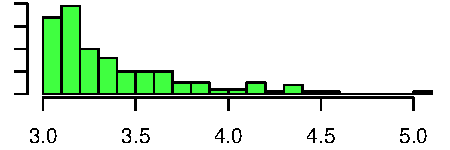
\includegraphics{quakes-mag-hist}
   \end{center}

   \alert{The distribution is skewed,} so with $n\approx 20$, the Normal assumption might not be good.

\end{frame}

%%%%%%%%%%%
\subsection{Transforming the data}

%%%%%%
\begin{frame}{Transformations}

    \begin{block}{Transforming the data}
        means applying a function to the data before doing statistics,\\
        for example
        \[  Y = \text{growth rate} \longrightarrow Y = \log( \text{growth rate} ). \]
    \end{block}

    \vspace{2em}

    \structure{Goal:} make the sampling distribution of $\bar Y$ closer to Normal,\\
    by making the population distribution of $Y$ closer to Normal.

    \vspace{2em}

    \structure{This is a good idea if}
    \begin{enumerate}
        \item The original data do not look Normally distributed,
        \item the transformed data look closer to Normal,
        \item and the statistics you are using require the sampling distribution of $\bar Y$ to be Normal.
    \end{enumerate}

    \vspace{2em}

    \structure{Remember:} informally, ``Normal'' means ``bell-shaped''.

\end{frame}

%
\begin{frame}{Example: earthquakes}

%      do.call( cbind, with( subset(quakes,MAG>3), tapply( log(MAG-3.0), weekdays(date), function (x) { list(n=length(x),mean=mean(x),sd=sd(x)) } ) ) )
%      Friday    Monday    Saturday  Sunday   Thursday  Tuesday   Wednesday
% n    21        24        31        22       23        24        21       
% mean -1.406708 -1.211826 -1.240581 -1.7097  -1.140423 -1.828194 -1.432289
% sd   0.984279  0.9498052 1.234087  1.158273 1.145213  1.35883   1.040219 
%      with( subset(quakes,MAG>3), t.test( log(MAG-3.0)[weekdays(date)=="Sunday"], log(MAG-3.0)[weekdays(date)=="Monday"] ) )
% t = -1.5858, df = 40.736, p-value = 0.1205
% alternative hypothesis: true difference in means is not equal to 0
% 95 percent confidence interval:
%  -1.1320528  0.1363043
% sample estimates:
% mean of x mean of y 
% -1.709700 -1.211826 
%   
%   pdf(file="quakes-log-mag-hist.pdf",width=3,height=1,pointsize=10)
%   par(mar=c(2,1,0,0)+.1)
%   hist( log(quakes$MAG[quakes$MAG>3]-3.0), breaks=25, col=adjustcolor("green",.75), main='', xlab='', ylab='' )
%   dev.off()

Earthquake \alert{$\log(\text{magnitude}-3.0)$}, for those above magnitude 3.0, on Sundays and Mondays in 2014:
  \begin{center}
    \begin{tabular}{crr}
       & Sundays & Mondays \\
       \hline
       $n$ & 22 & 24 \\
       $\bar y$ & -1.71 & -1.21 \\
       $s$ & 1.16 & 0.95
     \end{tabular}

   \vspace{2em}

   {$t_s=-1.60$ and $P=0.12$}\\
   CI for $\bar \mu_1 - \bar \mu_2$: $(-1.13,0.14)$
   \end{center}

   \pause 
   \begin{center}
     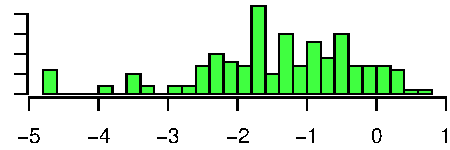
\includegraphics{quakes-log-mag-hist}
   \end{center}

   That looks \emph{closer} to bell-shaped.

\end{frame}


\subsection{Example by simulation}

%%%%%%
\begin{frame}{Real fake data:}
    
  \begin{center}
    (live simulation)
  \end{center}

\end{frame}



%%%%%% %%%%%%
\section{More about hypothesis testing}

\subsection{How to pick the hypotheses?}

%%%%%%
\begin{frame}{Hypotheses}

    Hypothesis testing requires 
    \begin{itemize}
        \item[$H_0$:] null hypothesis
        \item[$H_A$:] alternative hypothesis
    \end{itemize}

    \vspace{2em}

    \structure{Functional difference:} the null hypothesis is what you evaluate the $P$-value with.


\end{frame}


%%%%%%
\begin{frame}{A dialog}
    \begin{itemizew}{1em}
        \item[You:] It looks like $A$s are better than $B$s.  They tend to have more $X$.
        \item[Skeptic:] But what if they're the same, on average, you just happened to see more $X$ in your sample of $A$s?
        \item[You:] Ok, fine.  Suppose, for the sake of argument, that there \alert{isn't} a difference.
            Then let's see what the chance of seeing this much more $X$ is\ldots
    \end{itemizew}

    \vspace{2em}

    \structure{Note:}
    Often (like in this example), 
        \[ H_0: \mu_1 = \mu_2 , \]
    but not always.

\end{frame}


%%%%%%
\begin{frame}{What are the hypotheses?}

  To study the effect of latitude on body size in urban mammals, 
  we took two samples of mice, from Seattle and Los Angeles,
  and compared their mean body mass.

    \vspace{2em}
    \pause

  The El Ni\~no--Southern Oscillation (ENSO) effect produces increased rainfall along the entire Pacific coast about every four years.
  We collect rainfall data from many ENSO years, and compare the Seattle--Los Angeles difference to the usual level,
  knowing that Seattle gets on average 23 inches of rain per year more than Los Angeles.


    \vspace{2em}
    \pause

  We have genetic data from a genetic variant in 1,000 healthy people and 1,000 people with a disease,
  and would like to find out whether the genetic variant affects the chances of getting the disease.

\end{frame}



\subsection{Interpreting $P$-values}


%%%%%%
\begin{frame}{$P$-values}

    \begin{block}{}
      The \alert<1>{$P$-value} of a \alert<2>{result} is the probability of seeing a result \alert<3>{so extreme}, \alert<4>{if $H_0$ is true}.
    \end{block}

    \vspace{2em}
          \pause

    \begin{itemizew}{4em}
        \item[``result'':] the test statistic (ex: $\bar y_1 - \bar y_2$)
          \pause
        \item[``so extreme'':] defined by $H_A$ (ex: $\bar y_1 - \bar y_2 > C$)
          \pause
        \item[``if $H_0$ is true'':] how to compute the probability.
    \end{itemizew}

\end{frame}


\subsection{Medical testing example}

%%%%%%
\begin{frame}{Example:}

    A medical test for an illness:
    \begin{itemize}
        \item 1\% of population has the illness,
        \item 80\% chance of (true) detection if patient has the illness, 
        \item 5\% chance of (false) detection if patient does not.
    \end{itemize}

    \vspace{2em}

    With $H_0$: patient is healthy,
    if we test 1,000 patients, how many do we expect of:
    \begin{enumerate}
        \item falsely rejected null hypotheses? (type I errors)
        \item falsely accepted null hypotheses? (type II errors)
    \end{enumerate}

    \vspace{2em}
    \pause

    If you get a positive result,
    what's the chance that you have the illness?

    \vspace{2em}
    \pause

    \structure{True or false:} 
    We have found significant evidence for $H_A$ with $P<5\%$,
    so the probability that $H_0$ is true is 5\%.

    \vspace{2em}
    \pause

    What is a true statement similar to the above?


\end{frame}




\section<article>{Summary}
\section<presentation>*{Summary}

\begin{frame}{Summary}

    \begin{itemize}
        \item Statistical signficance \alert{does not imply} \\real--world significance.
        \item Lack of statistical signficance \alert{does not imply} \\real--world insignificance.
        \item Sample size acts like a \structure{magnifying glass}, making smaller differences visible.
        \item The \alert{effect size} describes the scale of a difference.
        \item Confidence intervals communicate both statistical signficance and real--world importance.
    \end{itemize}

    \vspace{1em}

  \begin{enumerate}
  \item The null hypothesis determines the conditions you use to calculate the $P$-value.
  \item If the conditions do not hold, the $P$-value may be wrong,
  \item or you might just be better off using a different test.
  \item The $t$-test depends on the sampling distribution of the sample mean being Normal;
  \item for this purpose, the closer the data are to Normal the better;
  \item sometimes, transforming the data helps.
  \end{enumerate}
\end{frame}

% homework
\begin{frame}{Homework}
  \begin{center}

  7.8.2

  \vspace{2em}

  7.9.1


  \end{center}
\end{frame}


\end{document}





